\documentclass[12pt]{article}
\usepackage[left=1in, right=1in, top=1in, bottom=1in]{geometry}
\usepackage{titling}

\usepackage{graphicx}
\usepackage[export]{adjustbox}
\usepackage{caption}
\usepackage{subcaption}
\usepackage{hyperref}

\hypersetup{
    colorlinks=true,
    linkcolor=blue,
    filecolor=magenta,      
    urlcolor=cyan,
}

\graphicspath{ {images/} }

\setlength{\droptitle}{-5em} 
\pretitle{\begin{center}\Huge\bfseries}
\posttitle{\par\end{center}\vskip 0.5em}
\preauthor{\begin{center}\Large\ttfamily}
\postauthor{\end{center}}
\predate{}
\postdate{}

\title{JumpMan \\ \large Interactive Graphics - Final project}
\author{Simone Bartolini 1752197}
\date{}
\begin{document}

\maketitle
\thispagestyle{empty}






\section{Libraries}
The game is developed in javascript using \href{https://threejs.org}{three.js} for 3D graphics. \href{https://github.com/SapienzaInteractiveGraphicsCourse/final-project-jumpman/blob/master/source/three.js-r118/examples/jsm/loaders/OBJLoader2.js}{OBJLoader2.js}, \href{https://github.com/SapienzaInteractiveGraphicsCourse/final-project-jumpman/blob/master/source/three.js-r118/examples/jsm/loaders/MTLLoader.js}{MTLLoader.js} and \href{https://github.com/SapienzaInteractiveGraphicsCourse/final-project-jumpman/blob/master/source/three.js-r118/examples/jsm/loaders/obj2/bridge/MtlObjBridge.js}{MtlObjBridge.js} from the three.js repository are also used for loading objects and materials and \href{https://github.com/SapienzaInteractiveGraphicsCourse/final-project-jumpman/blob/master/source/three.js-r118/examples/jsm/math/OBB.js}{OBB.js}, also from the three.js repository, is used for collision detection. Finally, \href{https://github.com/tweenjs/tween.js}{tween.js} is used for interpolation of animation keyframes. \\
The project contains various snippets of code from the \href{https://threejs.org/docs/index.html#manual/en/introduction/Creating-a-scene}{three.js documentation} and from the \href{https://threejsfundamentals.org}{threejsfundamentals.org} website as they have been my primary source for learning how to use three.js.

\section{Assets}
Various royalty-free assets have been used in this project: 
\begin{itemize}
\item The \textit{break.wav} sound effect has been obtained from \href{https://freesound.org/people/JustInvoke/sounds/446119/}{freesound.org} and created by user JustInvoke;
\item The \textit{crack.wav} sound effect is a cropped version of \textit{break.wav};
\item The \textit{hit.wav} sound effect has been obtained from \href{https://freesound.org/people/Cigaro30/sounds/420936/}{freesound.org} and created by user Cigaro30;
\item The \textit{spring.flac} sound effect has been obtained from \href{https://freesound.org/people/qubodup/sounds/172660/}{freesound.org} and created by users qubodup and cfork;
\item The \textit{breakableStepTopMap.png} texture has been obtained from \href{https://opengameart.org/content/light-wood-1024x1024}{opengameart.org} and created by user qubodup;
\item The \textit{breakableStepSideMap.png} texture is a cropped version of \textit{breakableStepTopMap.png};
\item The \textit{crackedStepTopMap.png} texture has been obtained by overlaying on top of \textit{breakableStepTopMap.png} \href{https://www.seekpng.com/ima/u2e6o0w7w7e6q8o0/}{this image from seekpng.com};
\item The \textit{crackedStepSideMap.png} texture has been obtained by overlaying on top of \textit{breakableStepSideMap.png} \href{https://www.pinclipart.com/maxpin/iiiJoi/}{this image from pinclipart.com};
\item The \textit{crackedStepSideNormalMap.png} and \textit{crackedStepTopNormalMap.png} textures have been generated from \href{https://www.pinclipart.com/maxpin/iiiJoi/}{this} and \href{https://www.seekpng.com/ima/u2e6o0w7w7e6q8o0/}{this} image respectively using \href{https://cpetry.github.io/NormalMap-Online/}{this tool} for generating normal maps;
\item The \textit{cloudMap.png} texture has been designed by me starting from \href{https://www.freepik.com/free-vector/clouds-background-flat-design_2040928.htm#page=1&query=cloud&position=6}{this image from freepik.com};
\item The \textit{columnNormalMap.png} texture is a cropped version of \href{https://1004259platformevaluation.files.wordpress.com/2011/12/pillarnormals.png}{this image from 1004259platformevaluation.wordpress.com};
\item The \textit{groundMap.png} texture has been obtained from \href{https://opengameart.org/content/tileable-bricks-ground-textures-set-1}{opengameart.org} and created by user Cethiel;
\item The \textit{movingStepMap.png}, \textit{movingStepNormalMap.png} and \textit{movingStepSpecularMap.png} textures have been obtained from this texture pack on \href{https://opengameart.org/content/metal-texture}{opengameart.org} created by user JosipKladaric;
\item The \textit{realStepMap.png} texture is a cropped version of \href{https://www.flickr.com/photos/seier/4357566390}{this image from flickr.com}, the \textit{realStepNormalMap.png} texture has been generated from the same image using \href{https://cpetry.github.io/NormalMap-Online/}{this tool} for generating normal maps.
\end{itemize}

\vspace{4mm}

Some of the assets have been created by myself, in particular:
\begin{itemize}
\item I have designed the \textit{starMap.png} texture using \href{https://affinity.serif.com/it/designer/}{Affinity Designer};
\item I have designed the \textit{hand.mtl}, \textit{hand.obj}, \textit{hand.png}, \textit{head.mtl}, \textit{head.obj}, \textit{head.png} materials, objects and textures using \href{https://ephtracy.github.io/}{MagicaVoxel} and taking inspiration from this model on \href{https://opengameart.org/content/hero-1}{opengameart.org} created by luckygreentiger.
\end{itemize}

\newpage

\section{Gameplay description}
The goal of the game is to climb a spiral staircase as high as possible without falling. The player character jumps automatically and by pressing the left or right arrow key, or by tapping the left or right side of the screen on touchscreen devices, the staircase rotates. To make the game more challenging there are various types of steps:
\\ \\
\renewcommand{\arraystretch}{3}
\begin{tabular}{p{13.5cm}p{2cm}}

\minipage{13cm} \renewcommand{\arraystretch}{1} \begin{tabular}{@{}p{2mm}p{12.5cm}@{}} • & \textbf{Normal steps:} as the name implies these steps act as one would expect, they are static and the player can jump in them as many times as he wants;\end{tabular}\endminipage 
& \minipage{2cm}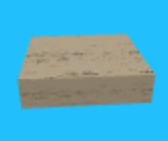
\includegraphics[width=2cm]{normal-step}\endminipage \\ 

\minipage{13cm} \renewcommand{\arraystretch}{1} \begin{tabular}{@{}p{2mm}p{12.5cm}@{}} • & \textbf{Moving steps:} these steps move up and down;\end{tabular}\endminipage 
& \minipage{2cm}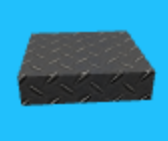
\includegraphics[width=2cm]{moving-step}\endminipage \\ 

\minipage{13cm} \renewcommand{\arraystretch}{1} \begin{tabular}{@{}p{2mm}p{12.5cm}@{}} • & \textbf{High jump steps:} these steps will make the player jump higher;\end{tabular}\endminipage
& \minipage{2cm}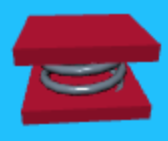
\includegraphics[width=2cm]{spring-step}\endminipage \\ 

\minipage{13cm} \renewcommand{\arraystretch}{1} \begin{tabular}{@{}p{2mm}p{12.5cm}@{}} • & \textbf{Breakable steps:} the player can jump on a breakable step only one time, the next time it will break;\end{tabular}\endminipage
& \minipage{2cm}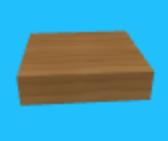
\includegraphics[width=2cm]{breakable-step}\endminipage \\ 

\minipage{13cm} \renewcommand{\arraystretch}{1} \begin{tabular}{@{}p{2mm}p{12.5cm}@{}} • & \textbf{Fading steps:} these steps fade in and out periodically, the player needs to time the jump right to avoid falling;\end{tabular}\endminipage
& \minipage{2cm}
\includegraphics[width=2cm]{fading-step}\endminipage \\ 

\minipage{13cm} \renewcommand{\arraystretch}{1} \begin{tabular}{@{}p{2mm}p{12.5cm}@{}} • & \textbf{Fake steps:} these steps have collision detection disabled, so the player needs to avoid them or he will fall.\end{tabular}\endminipage 
& \minipage{2cm}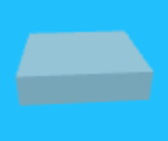
\includegraphics[width=2cm]{fake-step}\endminipage 

\end{tabular}
\renewcommand{\arraystretch}{1}

\newpage

\section{Technical description}

\subsection{Hierarchical models}

In the game there are two main hierarchical models, one for the player character and one for the staircase.

\subsubsection{Player character}
Figure \ref{fig:playerCharacter} illustrates the hierarchical model of the player character. The head and hands models are imported .obj files as described in the assets section. The torso, the feet and the upper and lower arms and legs are just simple box meshes. The container and the various pivots are THREE.Object3D() objects and are used to define the relative positions of the various parts of the model and the rotation points used for the animations.

\begin{figure}[h]
\centering
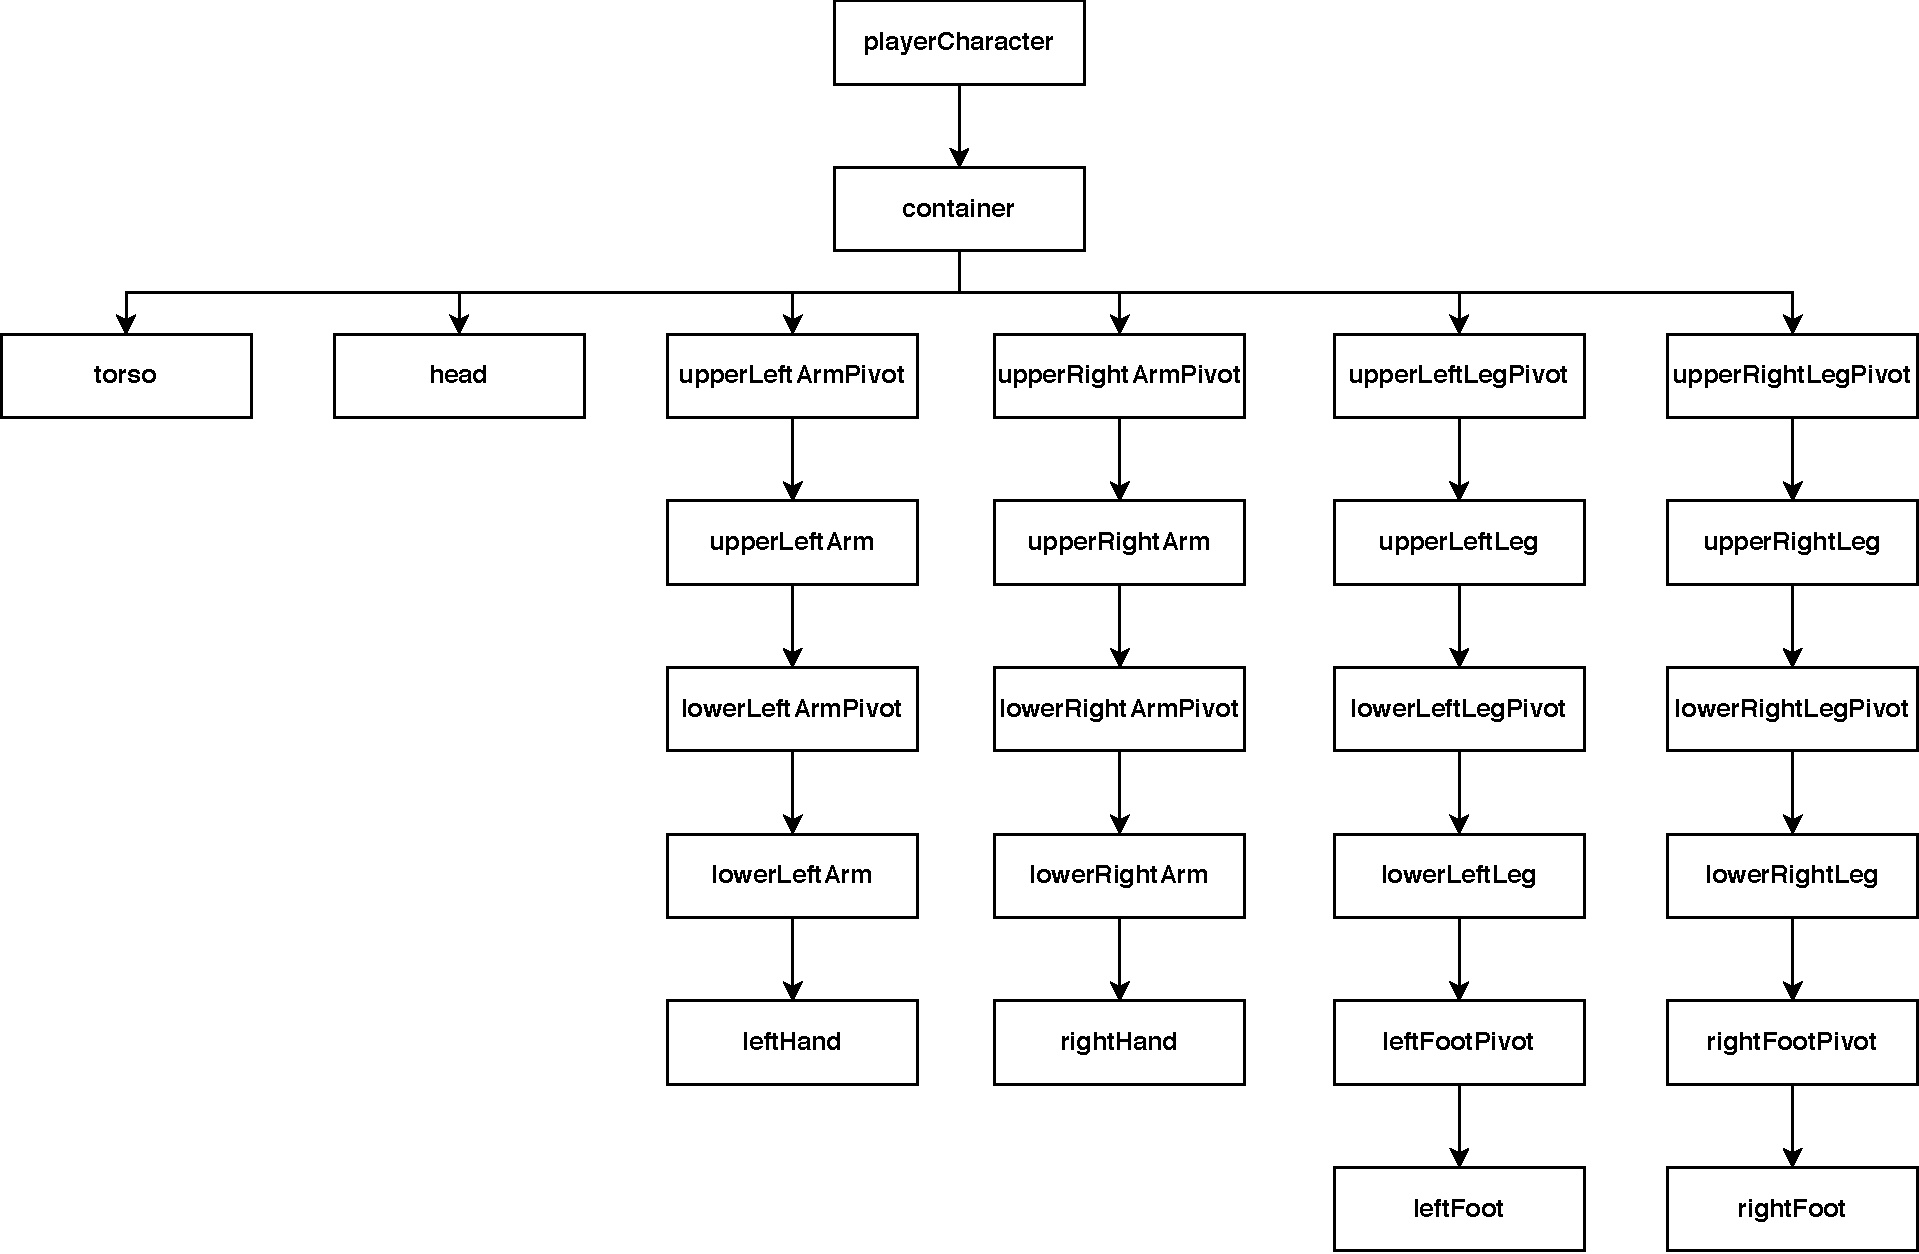
\includegraphics[width=\linewidth]{PlayerCharacter}
\caption{PlayerCharacter hierarchical model}
\label{fig:playerCharacter}
\end{figure}

\subsubsection{Staircase}

Figure \ref{fig:staircase} illustrates the hierarchical model of the staircase. It is composed of a central column, which is a simple cylindrical mesh, and a series of steps, with every step being a child of a THREE.Object3D() object called pivot that is used to define the position and rotation of the step relative to the center of the column.

\begin{figure}[h]
\centering
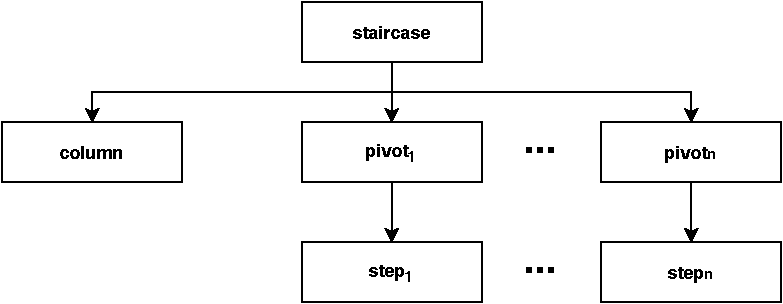
\includegraphics[width=0.7\linewidth]{staircase}
\caption{Staircase hierarchical model}
\label{fig:staircase}
\end{figure}


The type of each step in the ladder is selected probabilistically by the stepTypeGenerator object. The different types have different odds of being selected and the probabilities change as the player progresses in the game to increase the challenge.\\
The model of each step depends on the type: normal steps, moving steps, fading steps, fake steps and breakable steps (when not broken) are simple box meshes. When a breakable step is broken it is replaced with a new model, called brokenStep, which is made of two halves that are extruded, using three.js' ExtrudeBufferGeometry class, from a flat shape having a sawtooth pattern on the cracked side (Figure \ref{fig:brokenStep}). The high jump step instead is made of three parts, a top and a bottom box mesh and a central spring mesh, which is created using three.js' TubeBufferGeometry class (Figure \ref{fig:sprintStep}).

\begin{figure}[h]
\centering
\begin{subfigure}{.5\textwidth}
  \centering
  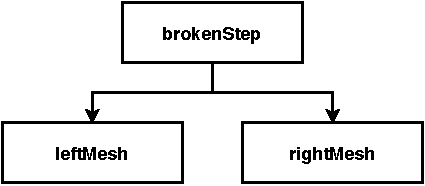
\includegraphics[width=.8\linewidth]{brokenStep}
  \caption{brokenStep hierarchical model}
  \label{fig:sub1}
\end{subfigure}%
\begin{subfigure}{.5\textwidth}
  \centering
  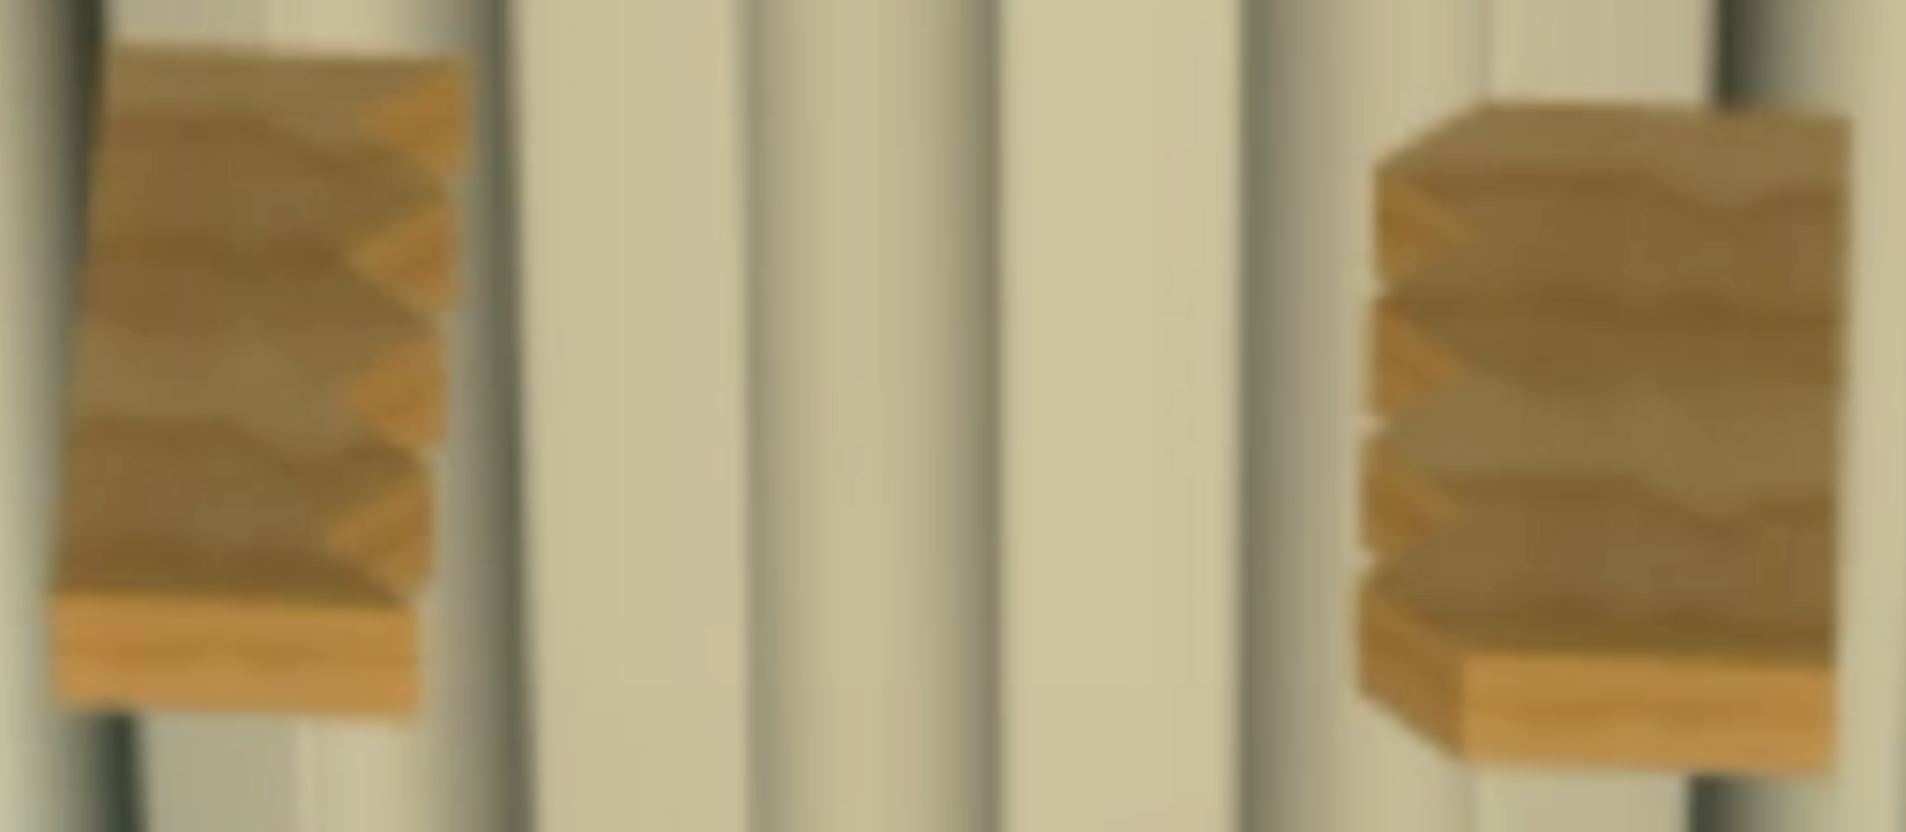
\includegraphics[width=.8\linewidth]{broken-step}
  \caption{The two halves of the brokenStep}
  \label{fig:sub2}
\end{subfigure}
\caption{brokenStep}
\label{fig:brokenStep}
\end{figure}

\begin{figure}[h]
\centering
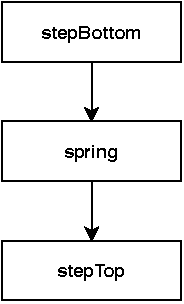
\includegraphics[width=0.18\textwidth]{springStep}
\caption{High jump hierarchical model}
\label{fig:sprintStep}
\end{figure}

\newpage

\subsection{Other objects}
\subsubsection{Ground and Fog}
The ground is just a simple plane with a flat shaded texture on top. To hide the seam between the ground and the sky a linear fog is used (Figure \ref{fig:ground-fog}).

\begin{figure}[h]
\centering
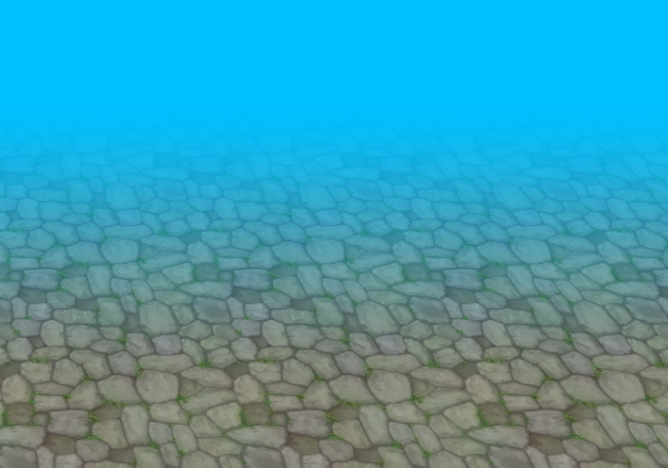
\includegraphics[width=0.7\textwidth]{ground-fog}
\caption{Ground and fog}
\label{fig:ground-fog}
\end{figure}

\subsubsection{Clouds}
To simulate the player going higher in the sky, clouds appear once reached a height of around 200 (Figure \ref{fig:clouds}). The clouds are not a 3D model but just a plane with a flat shaded texture on top, oriented to always look a the camera.
\begin{figure}[h]
\centering
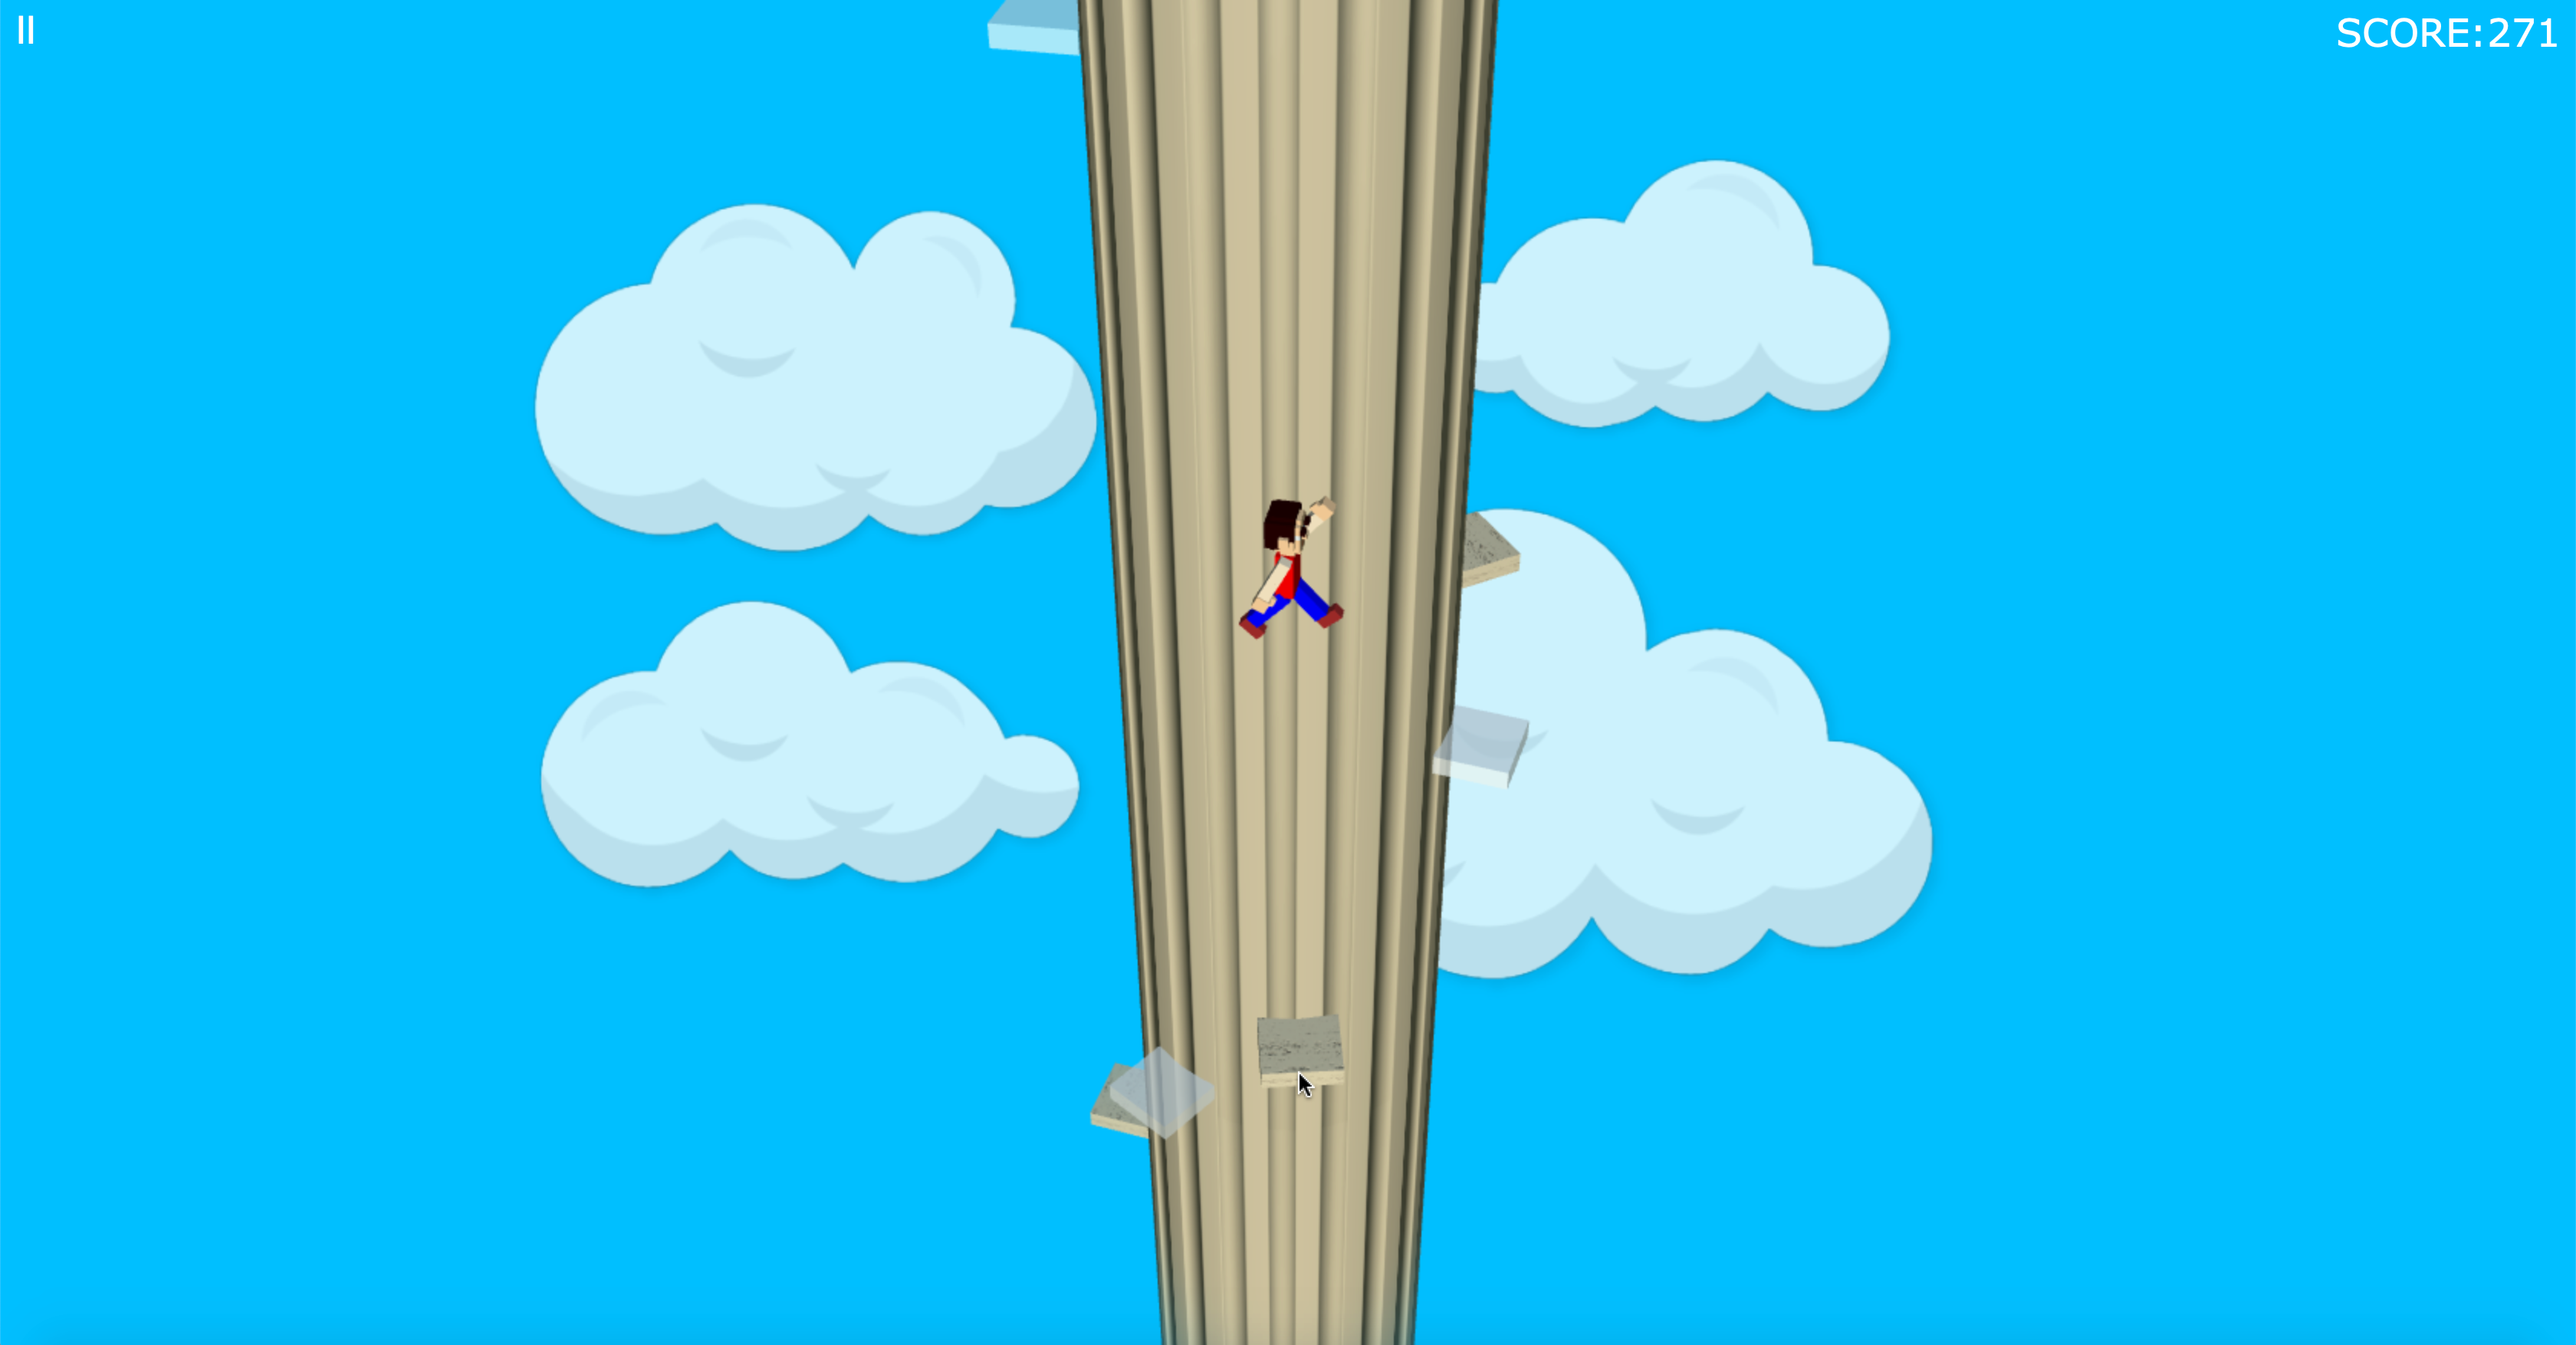
\includegraphics[width=0.7\textwidth]{clouds}
\caption{Clouds}
\label{fig:clouds}
\end{figure}

\subsubsection{Stars}
At a height of around 700 the sky color starts getting darker and stars appear in the sky to simulate the player going into space (Figure \ref{fig:stars}). The stars are rendered using the three.js particles system.

\begin{figure}[h]
\centering
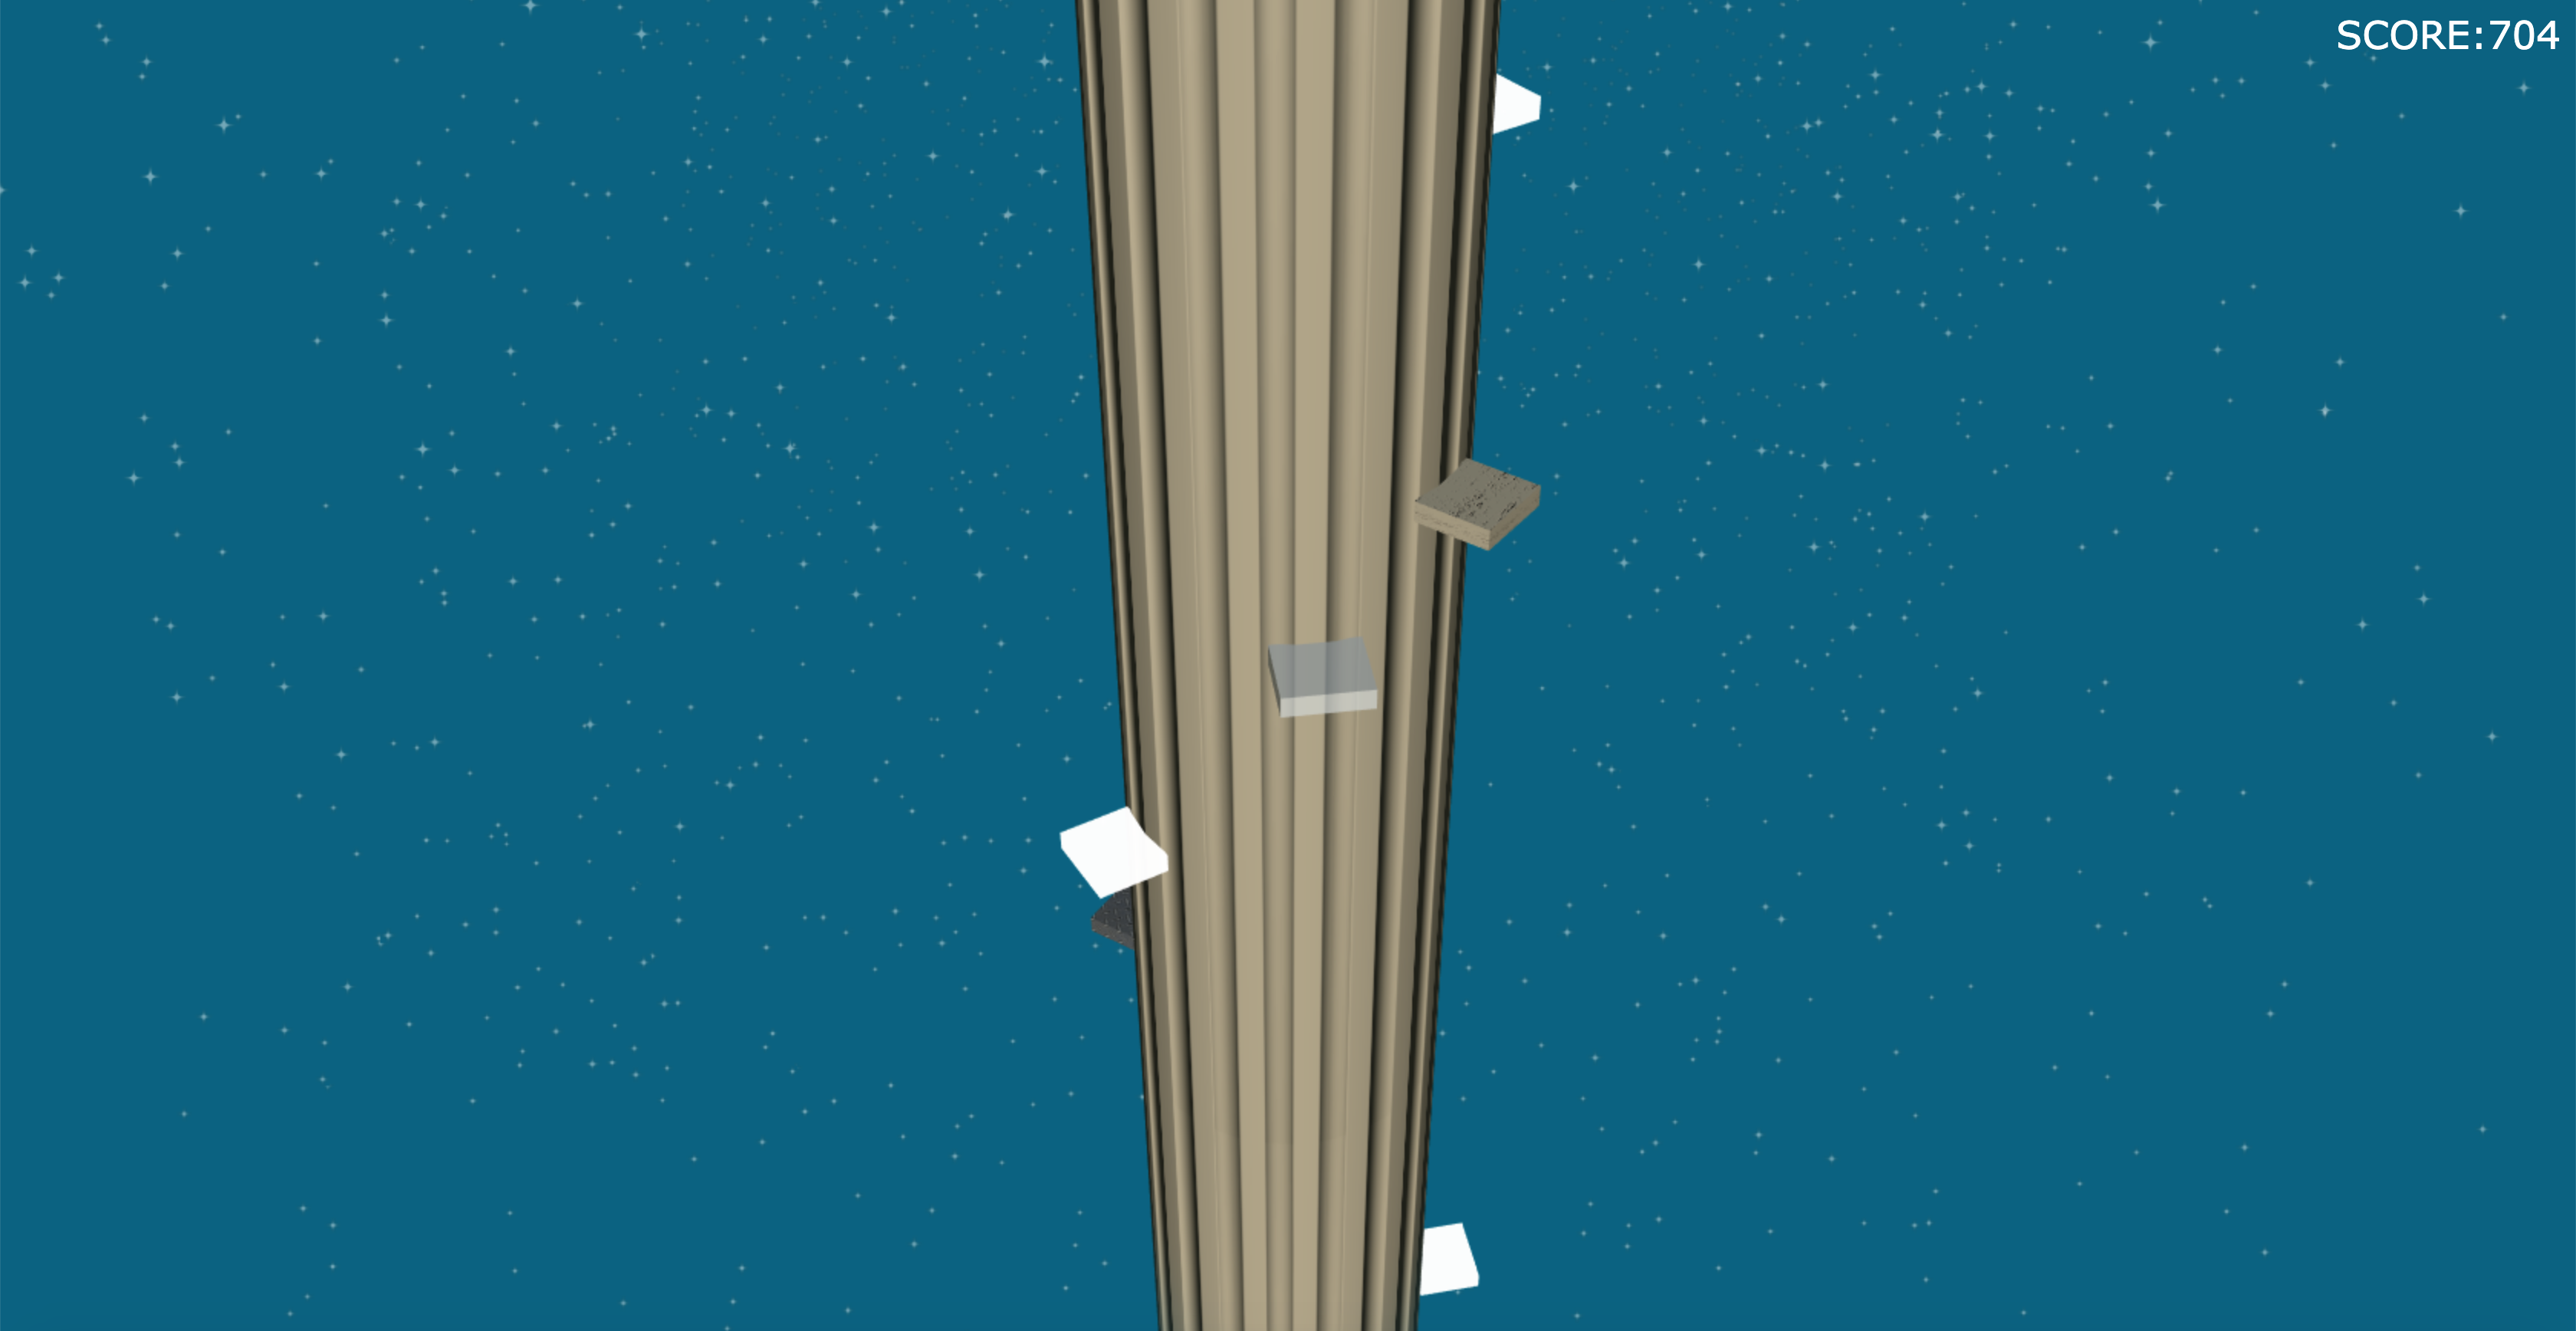
\includegraphics[width=0.7\textwidth]{stars}
\caption{Stars}
\label{fig:stars}
\end{figure}

\subsection{Lighting and textures}
Every object, except the ground and the clouds, is shaded using Phong shading. There are two lights: a directional light and a hemisphere ambient light. The two colors of the hemisphere light, together with the background color, slowly change as the player climbs the ladder to simulate the player leaving the atmosphere and going into space. 
As for the textures, various types are used for different objects:
\begin{itemize}
\item the head and hands models of the player character use the color textures exported from MagicaVoxel together with the .mlt and .obj files, while the other parts of the character have just a color assigned (i.e. no texture is used);
\item the column has a beige color assigned, to mimic marble, plus a normal map is used to replicate the grooves of a classical column;
\item the normal steps are designed to look like if they are made out of travertine, thus the same beige color of the column is used plus a color and a normal texture to mimic the imperfections of travertine;
\item the moving steps use a color, a normal and a specular map to make them look like they are made out of metal;
\item the breakable steps use color textures to mimic wood. Once the player jumps on one of them for the first time, the color textures are swapped and a normal map is added to make it appear that the wood has cracked;
\item as said before the ground and the clouds are rendered using a flat shaded color texture;
\item a color texture is used to make the particles look like stars in the sky.
\end{itemize}
Fading, fake and high jump steps have no texture, just basic colors assigned but:
\begin{itemize}
\item the high jump steps have a high shininess value to make the top and bottom part look like plastic and the central spring look like polished metal;
\item fake steps have an opacity value of 0.7 to make them look slightly transparent;
\item fading steps are emissive.
\end{itemize}




\subsection{Animations}
\subsubsection{Staircase}
As said before, the player controls the rotation of the staircase by pressing the left or right key or by tapping on the left or right side of a touchscreen device. In particular when the player press left or right the value 1 or -1 is assigned to a variable called \textit{move}. When the player stops pressing the button (or touching the screen) the variable \textit{move} is reinitialized back to 0. At each frame of the game the value \(0.02 * move\) is added to the rotation on the \textit{y} axis of the staircase. \\
When a collision is detected between the player character and a step that is higher than the previous one the camera is moved up. The animation of the camera movement is eased using tween.js and the quadratic ease-out function. Since the player could in theory continue climbing the ladder without falling for an infinite amount of time we will need an infinitely long staircase. To solve this problem the central column of the staircase is designed to be a little bit longer than the screen height and is moved up together with the camera to fake it being infinite (except for the first part of the game when the ground is still visible, moving the column at that time would break the illusion). Also every time a step goes out of frame it is removed while new steps are added on top of the staircase. \\
Tween.js is also used to animate the moving, fading, breakable, and high jump steps in particular:
\begin{itemize}
\item the moving steps move up and down repeatedly by 5 points with a quadratic in-out easing function;
\item the opacity of fading steps goes repeatedly from 1 to 0 and back to 1 with an exponential in-out easing function;
\item when a breakable step is broken the two halves of the broken step are animated to fall down and move away from each other;
\item when the player jumps on a high jump step the spring is compressed, then extended and then it goes back to the initial state.
\end{itemize}


\subsubsection{Player character}
The animation of the player character is divided into two cycles, one defining the up and down movement of the jump and the other defining the pose during the jump. The game starts with the player character already in the air and falling down to the ground. At the beginning it falls by 15 points using a quadratic ease-in function (simulating gravity), then it continues falling at a constant speed (simulating having reached terminal velocity). Once a collision with a step is detected, the falling animation is stopped and the jumping animation starts, i.e the character goes up by 15 points (or by 44 points if it stepped on a high jump step) using a quadratic ease-out function. Once reached the end of the jumping animation, the falling animation will be restarted. In the meantime the character changes pose, interpolating between three keyframes (Figure \ref{fig:keyframes}). The character starts on keyframe 1 (Figure \ref{fig:key1}), then while falling switches to keyframe 2 (Figure \ref{fig:key2}) and then goes to keyframe 3 (Figure \ref{fig:key3}) when colliding with a step. After that it goes back to keyframe 2 (Figure \ref{fig:key2}) and then to keyframe 1 (Figure \ref{fig:key1}) once reached the apex of the jump.

\begin{figure}[h]
\centering
\begin{subfigure}{.33\textwidth}
  \centering
  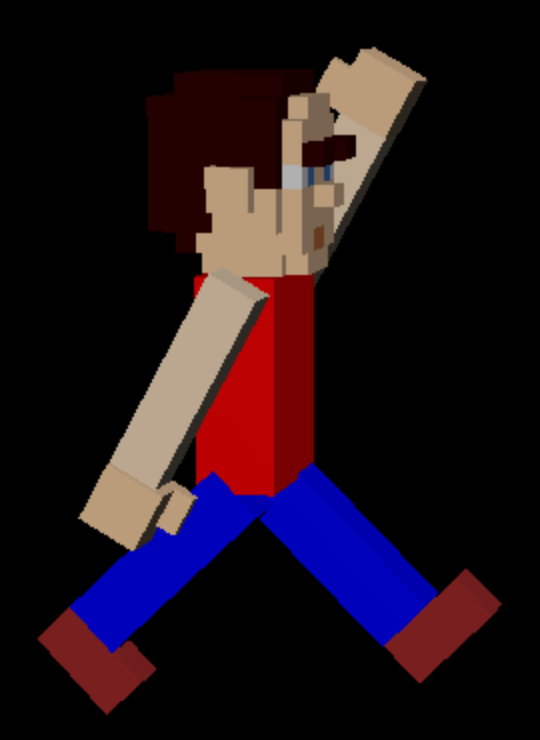
\includegraphics[width=.9\linewidth]{1}
  \caption{Keyframe 1}
  \label{fig:key1}
\end{subfigure}%
\begin{subfigure}{.33\textwidth}
  \centering
  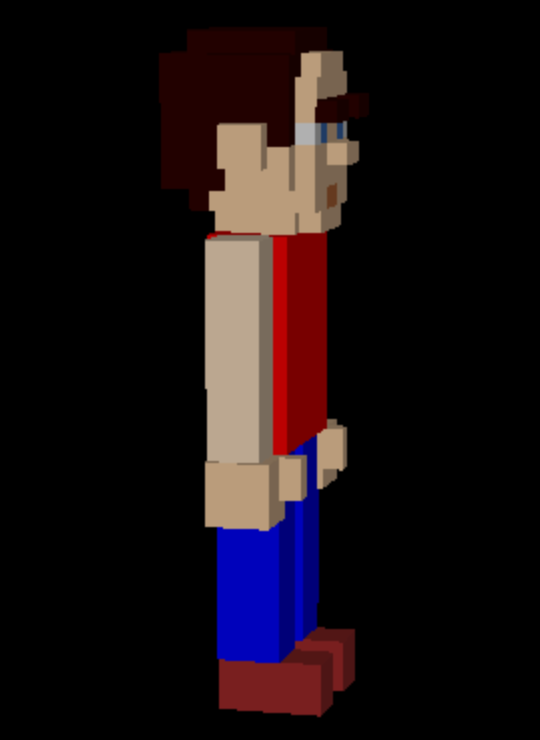
\includegraphics[width=.9\linewidth]{2}
  \caption{Keyframe 2}
  \label{fig:key2}
\end{subfigure}%
\begin{subfigure}{.33\textwidth}
  \centering
  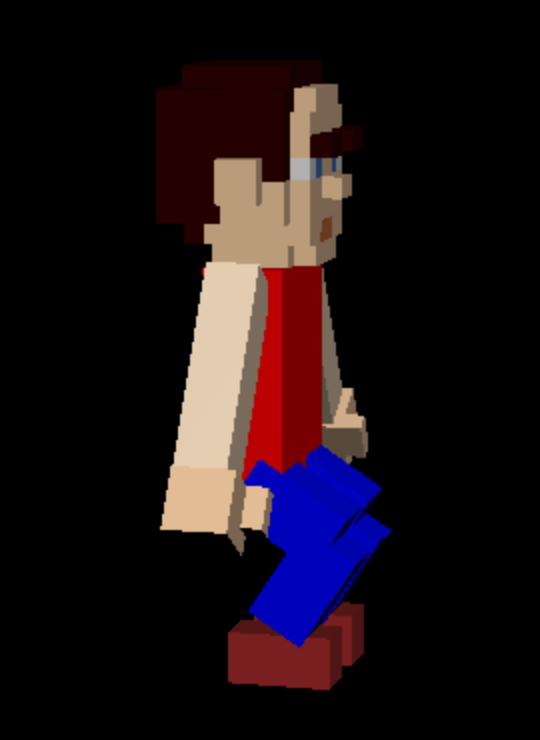
\includegraphics[width=.9\linewidth]{3}
  \caption{Keyframe 3}
  \label{fig:key3}
 \end{subfigure}
\caption{Keyframes of the jumping animation}
\label{fig:keyframes}
\end{figure}

\newpage

\section{Other notable stuff}

\subsection{Preloading}
To avoid stuttering every time a new step type appears in the game the steps materials and geometries are preloaded in the first frame of the game, by adding and then immediately removing the steps and positioning them out of the view frustum to ensure they are not visible, so that the relative shaders are compiled and the data sent to the GPU.

\subsection{Tutorial}
The tutorial page explains the rules of the games and shows the various steps types. This page is heavily inspired by \href{https://threejsfundamentals.org/threejs/lessons/threejs-multiple-scenes.html}{this guide on threejsfundamentals.org} on how to have multiple scenes in an html page, aligned with the text of the page. In this case the technique is used to draw the various step types near their relative description.

\subsection{Leaderboard}
The game has also a simple local leaderboard. At the end of a game the player can save the score, which will be added in the browser cookies. When the player access the \textit{Leaderboard} page the scores will be retrieved from the cookies.

\end{document}